\documentclass[12pt]{article}

\usepackage[utf8]{inputenc}
\usepackage[margin = 1in]{geometry}
\usepackage[english]{babel}
\usepackage{amsthm}
\usepackage{amssymb}
\usepackage{amsmath}
\usepackage{changepage}
\usepackage[makeindex]{imakeidx}
\usepackage{textcomp}
\usepackage{gensymb}
\usepackage{xcolor, soul}
\usepackage{hyperref}
\usepackage{parskip}
\usepackage{graphicx}

\graphicspath{ {./images/} }

\definecolor{linkColour}{RGB}{140, 25, 57}
\definecolor{urlColour}{RGB}{137, 62, 27}

\hypersetup{
    colorlinks,
    citecolor=purple,
    filecolor=purple,
    linkcolor=linkColour,
    urlcolor=urlColour
}

\makeindex

\newcommand{\homl}{\hyperlink{homl}{Hands-On Machine Learning}}

\newenvironment{fact*}[2][]
    {
    \begin{adjustwidth}{1em}{0em}
    \noindent
    \textbf{#2} \hfill #1
    
    \vspace{0.1in}
    \noindent
    \ignorespaces
    }
    {
    \end{adjustwidth}
    }

\newenvironment{fact}[2][]
    {
    \index{#2}
    \hypertarget{#2}{\vspace{0.2in}}
    \begin{adjustwidth}{1em}{0em}
    \noindent
    \textbf{#2} \hfill #1
    
    \vspace{0.1in}
    \noindent
    \ignorespaces
    }
    {
    \end{adjustwidth}
    }

\title{Companion to Machine Learning}
\author{Rohan Kumar}
\date{}






\begin{document}

\maketitle
\newpage
\tableofcontents
\newpage

\section*{Introduction}

\subsection{What is Machine Learning}
    Machine Learning is the field of study that gives computers the ability to learn from data without being 
    explicitly programmed. This is good for problems that require a lot of fine-tuning or for which using a 
    traditional approach yields no good solution. Machine Learning's data dependency allows it to adapt to new data
    and gain insight for complex problems and large amounts of data.

\subsection{Applications of Machine Learning}
    Machine Learning can be used for a range of tasks and can be seen used in:
    \begin{itemize}
        \item Analyzing images of products on a production line to automatically classify them (Convolutional Neural Net)
        \item Forecasting company revenue based on performance metrics (Regression or Neural Net)
        \item Automatically classifying news articles (NLP using Recurrent Neural Networks)
        \item Summarizing long documents automatically (Natural Language Processing)
        \item Building intelligent bot for a game (Reinforcement Learning)
    \end{itemize}

\subsection{Types of Machine Learning}
    \begin{fact}[\homl]{Supervised Learning}
        In supervised learning, the training set you feed to the algorithm includes the desired solutions, called labels.
        (e.g determining if an email is spam would be trained a dataset of example emails labelled as spam or not spam.) \\[0.1in] 
        Some commonly used supervised learning algorithms are:
        \begin{itemize}
            \item k-Nearest Neighbors
            \item Linear Regression
            \item Logistic Regression
            \item Support Vector Machines (SVMs)
            \item Decision Trees and Random Forests
            \item Neural Networks
        \end{itemize}
    \end{fact}

    \begin{fact}[\homl]{Unsupervised Learning}
        In unsupervised learning, the training data is unlabeled and the system tries to learn without guidance. The system
        will try and automatically draw inferences and conclusions about the data and group it as such. (e.g. having a lot of
        data about blog visitors. Using a clustering algorithm we can group and detect similar visitors). \\[0.1in]
        Some important unsupervised learning algorithms are:
        \begin{itemize}
            \item Clustering
            \begin{itemize}
                \item K-Means
                \item DBSCAN
                \item Hierarchical Cluster Analysis
            \end{itemize}
            \item Anomaly detection and novelty detection
            \begin{itemize}
                \item One-class SVM
                \item Isolation Forest
            \end{itemize}
            \item Visualization and dimensionality reduction
            \begin{itemize}
                \item Principal Component Analysis (PCA)
                \item Kernel PCA
                \item Locally Linear Embedding (LLE)
                \item t-Distributed Stochastic Neighbor Embedding (t-SNE)
            \end{itemize}
            \item Association rule learning
            \begin{itemize}
                \item Apriori
                \item Eclat
            \end{itemize}
        \end{itemize}
    \end{fact}

    \begin{fact}[\homl]{Semisupervised Learning}
        Labelling can be very time-consuming and costly, often there will be plenty of unlabelled and a few labelled instances.
        Algorithms that deal with data that is partially labeled is called semi-supervised learning. A good example of this is
        Google Photos. Google clusters and groups your photos based on facial recognition (unsupervised) and then you can label one photo and it
        will be able to label every picture like that (supervised). Most semi-supervised learning algorithms are combinations of unsupervised and 
        supervised algorithms.  
    \end{fact}

    \begin{fact}[\homl]{Reinforcement Learning}
        Reinforcement Learning is a learning algorithm based on a reward system. The learning system, called an agent, can observe the environment,
        select and perform actions, and get rewards in return (or penalties in the form of negative rewards). It will then learn by itself what the 
        best strategy, called a policy, to get the most reward over time. A policy defines what action the agent should choose when it is in a given
        situation.
    \end{fact}

\newpage

\section*{Sources}
    Throughout this compendium, each piece of information will be formatted as such.
    
    \vspace{0.1in}
    \begin{fact*}[Source]{Name / Description of fact}
        Information about fact.
    \end{fact*}
    \vspace{0.3in}
    
    \noindent The location which currently contains ``Source'' could potentially be filled with a variety of sources. Here is how to find the source based off the shortened form.
    
    \begin{itemize}
        \item \hypertarget{homl}{\textbf{Hands-On Machine Learning}} refers to Hands-On Machine Learning with Scikit-Learn, Keras, and TensorFlow, 2nd Edition by Aurélien Géron
    \end{itemize}

\newpage

\section{Data Analysis}
TODO:
\begin{itemize}
    \item Data Model
    \item Overfitting/Underfitting
    \item Feature Normalization
    \item Types of Loss Functions
\end{itemize}

\section{Activation Functions}
    \subsection{Sigmoid Function}
        The \textit{sigmoid function} denoted $\sigma(\cdot)$ outputs a number between 0 and 1. It is defined as
        $$ \sigma(t) = \frac{1}{1 + exp(-t)} $$
        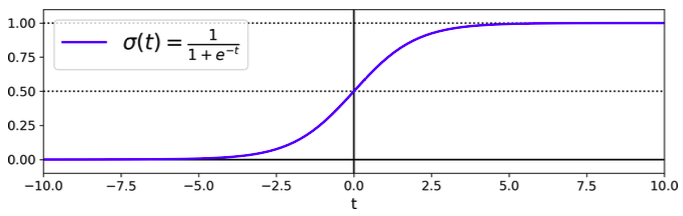
\includegraphics[scale=0.7]{sigmoid}

        The key property of the sigmoid function is that $\sigma(t) < 0.5$ when $t < 0$, and $\sigma(t) \geq 0.5$ when $t \geq 0$, so a sigmoid function is useful for classification since it can predict 1 when $\boldsymbol{w}^T\boldsymbol{x}$
        is positive and 0 if it is negative.

\section{Convex Optimization}
    TODO:
    \begin{itemize}
        \item Gradient Descent
        \item Normal Solution
        \item Other methods e.g Newtons Method
    \end{itemize}

\section{Statistical Learning}
    Data is often incomplete, indirect, or noisy. Statistical learning lets us consider forms of uncertainty to help us build better models.

    \subsection{Bayesian Learning}
    Bayes' theorem describes the probability of an event $H$ given evidence $e$.
    \begin{align}
        P(H|e) &= \frac{P(e|H)P(H)}{P(e)} \\
        &= kP(e|H)P(H)
    \end{align}

    where:
    \begin{itemize}
        \item $P(H|e)$: Posterior probability
        \item $P(e|P)$: Likelihood
        \item $P(H)$: Prior probability
        \item $P(e)/k$: Normalizing constant
    \end{itemize}

    Bayesian Learning consists of determining the posterior probability using Bayes' theorem.
    
    Suppose we want to make a prediction about an unknown quantity X we can consider the hypothesis space which represents all possible models $h_i$ to predict the scenario.

    \begin{align}
        P(X|\boldsymbol{e}) &= \sum_i P(X|e, h_i)P(h_i|e) \\
        &= \sum_i P(X|h_i)P(h_i|e)
    \end{align}

    This prediction yields the weighted combination of all the hypothesis' in the hypothesis space based on it's likelihood from the evidence. The prior $P(h_i | e)$ is yields the weight for each hypothesis and $P(X|h_i)$ yields the likelihood
    of the hypothesis for the unknown quantity $X$.

    Bayesian probability is:
    \begin{itemize}
        \item Optimal: give a prior probability, no prediction is correct more often than the Bayesian prediction.
        \item Overfitting-free: all hypothesis are weighted and considered, eliminating overfitting.
    \end{itemize}

    One of the constraints of bayesian learning is that it can be intractable when the hypothesis space grows very large, often as a result of approximating a continuous hypothesis space with many discrete hypothesis. This requires us to approximate 
    Bayesian Learning.

    \subsection{Approximate Bayesian Learning}
    \subsubsection{Maximum a Posteriori}
        Maximum a Posteriori (MAP) makes predictions based on only the most probable hypothesis $h_{MAP} = argmax_{h_i}P(h_i | e)$. This differs from Bayesian learning, which makes predictions for all hypothesis weighted by their probability. 
        MAP and Bayesian learning predictions tend to converge as the amount of data increases, and overfitting can be mitigated by giving complex hypothesis a low prior probability. However, finding $h_{MAP}$ may be difficult or intractable.

    \subsubsection{Maximum Likelihood}
        Maximum Likelihood (ML) simplifies MAP by assuming uniform prior probabilities and then makes a prediction based on the most probable hypothesis $h_{ML}$. ML tends to be less accurate than MAP and Bayesian predictions, it is also subject to overfitting
        due to the prior probabilities being uniform. Finding $h_{ML}$ is easier than finding $h_{MAP}$ since finding $h_{ML}$ for $P(e|h)$ is equivalent to calculating it for $argmax_h \sum_n logP(e_n |h)$.

\section{Linear Models}
    \subsection{Linear Regression}
    \subsubsection{Formulation}
        Linear Regression is a supervised machine learning algorithm where the predicted output is continuous and has a constant slope. Our main objective is to generate a line that
        minimizes the distance from the line to all of data points. This is essentially minimizing the error and maximizing our prediction accuracy.
    
    \subsubsection{Simple Regression}
        A simple two variable linear regression uses the slope-intercept form, where $m$ and $b$ are the variables our algorithm will try to "learn". $x$ represents our input data
        and $y$ represents the prediction.
        $$ y = mx + b$$

    \subsubsection{Multivariable Regression}
        Often times there are more than one feature in the data and we need a more complex multi-variable linear equation as our hypothesis. We can represent our hypothesis with the
        follow multi-variable linear equation, where $\boldsymbol{w}$ are the weights and $\boldsymbol{x}$ is the input data.

        \begin{align*}
            h_{\boldsymbol{w}}(\boldsymbol{x}) &= w_0x_0 + w_1x_1 w_2x_2 + ... + w_nx_n \\
            &= \boldsymbol{w}^T\boldsymbol{x}
        \end{align*}

    \subsubsection{Cost Function}
        To predict based on a dataset we first need to learn the weights that minimize the mean squared error (euclidean loss) of our hypothesis. We can define the following to be our cost function to
        minimize with $m$ being the number of data points and $i$ being the $i^{th}$ training example.
        \begin{align*}
            J(\boldsymbol{w}) &= \frac{1}{2m}\sum_{i=1}^{m}(h_{\boldsymbol{w}}(\boldsymbol{x}^i) - y^i)^2 \\
            &= \frac{1}{2m}(X\boldsymbol{w} - \boldsymbol{y})^T(X\boldsymbol{w} - \boldsymbol{y})
        \end{align*}


    \subsubsection{Gradient Descent Solution}
        Now to solve for $\boldsymbol{w}$ we can use Gradient Descent and iteratively update $\boldsymbol{w}$ until it converges. We get the slope of the cost function to be:
        $$ \frac{\partial J{\boldsymbol{w}}}{\partial \boldsymbol{w}_j} = \frac{1}{m}\sum_{i=1}^m(\boldsymbol{w}^T\boldsymbol{x}^{i}-y^{i})\boldsymbol{x}_{j}^i $$
        now applying a step $\alpha$ we can iteratively change $\boldsymbol{w}$ until it reaches the global minima. 
        $$ \boldsymbol{w}_j := \boldsymbol{w}_j - \alpha \frac{1}{m}\sum_{i=1}^{m}(h_{\boldsymbol{w}}(\boldsymbol{x}^i) - y^i) $$

    \subsubsection{Normal Equation Solution}
        The closed form solution to the linear system in $\boldsymbol{w}$
        $$ \frac{\partial J{\boldsymbol{w}}}{\partial \boldsymbol{w}_j} = \frac{1}{m}\sum_{i=1}^m(\boldsymbol{w}^T\boldsymbol{x}^{i}-y^{i})\boldsymbol{x}_{j}^i = 0 $$
        writing this as a linear system in $w$ we get $A\boldsymbol{w} = b$ where
        $$ A = \sum_{n=1}^N(\boldsymbol{x}_n \boldsymbol{x}_n^T) \ \textrm{and} \ b = \sum_{n=1}^N(\boldsymbol{x_n} y_n) $$
        so we can solve for $\boldsymbol{w} = \boldsymbol{A}^{-1}\boldsymbol{b}$ and get the following vectorized solution.
        $$ \boldsymbol{w} = (X^TX)^{-1}X^T\boldsymbol{y} $$
    
    \subsection{Logistic Regression}
        \subsubsection{Formulation}
            Logistic regression is an algorithm used for classification. It is used to estimate the probability that an instance belongs to a particular class. If the estimated probability is
            greater than 50\%, then the model predicts the instance belongs to that class, and otherwise it predicts it does not. This makes it a binary classifier.

        \subsubsection{Prediction}
            Logistic Regression computers the weighted sum of the input features (plus a bias term) and outputs the logistic (\hyperlink{sigmoid function}{Sigmoid Function}) of the result. The hypothesis is given by
            $$ p = h_{\boldsymbol{w}}(\boldsymbol{x}) = \sigma(\boldsymbol{w}^T\boldsymbol{x}) $$
            
            Once the Logistic Regression model has estimated the probability that an instance $boldsymbol{x}$ belongs to the positive class, it can make its prediction $y$ easily.
            \[ y = 
                \begin{cases} 
                    0 & p < 0.5 \\
                    1 & p\geq 0.5 
                \end{cases}
            \]
        
        \subsubsection{Cost Function}
            The objective of training the model is such that the model estimates high probabilities for positive instances $(y = 1)$ and low probabilities for negative instances $(y = 0)$.
            This concept is captured through the cost function shown below.
            \[ J(\boldsymbol{w}) = 
                \begin{cases}
                    -log(p) & y = 1 \\
                    -log(1-p) & y = 0
                \end{cases}
            \]
            
            This makes intuitive sense because $-log(t)$ grows very large when $t$ approaches 0, so the cost will be large if the model estimates a probability close to 0 for a positive instance.
            The cost will also be very large if the model estimates a probability close to 1 for a negative instance. On the other hand $-log(t)$ is close to 0 when $t$ is close to 1, so the cost
            will be close to 0 if the estimated probability is close to 0 for a negative instance or close to 1 for a positive instance.

            We can express the cost as a single expression called the \textit{log loss}. 

            $$J(\boldsymbol{w}) = -\frac{1}{m}\sum_{i=1}^m[y^{(i)} log(h_{\boldsymbol{w}}(\boldsymbol{x}^{(i)})) + (1-y^{(i)}log(1-h_{\boldsymbol{w}}(\boldsymbol{x}^{(i)}))] $$

        \subsubsection{Solution}
            Unfortunately, there is no known closed-form solution to compute the value of $\boldsymbol{w}$ that minimizes the cost function. The cost function however, is convex, so Gradient Descent or 
            any other optimization algorithm is guaranteed to find the global minimum. The gradient can be expressed as:

            $$ \frac{\partial J{\boldsymbol{w}}}{\partial \boldsymbol{w}_j} = \frac{1}{m}\sum_{i=1}^m(\sigma(\boldsymbol{w}^T\boldsymbol{x}) - y^{(i)} x_j^{(i)}) $$
            
            Some faster more sophisticated methods are
            \begin{itemize}
                \item Conjugate Gradient
                \item BFGS
                \item L-BFGS
            \end{itemize}

        \subsubsection{Softmax Regression}
            The Logistic Regression model can be generalized to support multiple classes. When given an instance $\boldsymbol{x}$, the Softmax Regression model computes a score $s_k(\boldsymbol{x})$ for each class $k$,
            then estimates the probability of each class by applying the \textit{softmax function} to the scores. 

            $$ s_k(\boldsymbol{x}) = \boldsymbol{w}^T_k\boldsymbol{x} $$

            Once the score of every class for the instance $\boldsymbol{x}$ is computed, you can estimate the probability $p_k$ that the instance belongs to class $k$. The function computes the exponential of each score, 
            the normalizes them.

            $$ p_k = P(y^{(i)} = k | \boldsymbol{x}^{(i)}, \boldsymbol{w}) = \frac{exp(s_k(\boldsymbol{x}))}{\sum_{j=1}^K exp(s_j(\boldsymbol{x}))} $$

            The Softmax Regression classifier predicts the class with the highest estimated probability.

            The cost function associated with the Softmax Regression Classifier is the Cross Entropy cost function; it penalizes the model when it estimates a low probability for a target class. Cross entropy is used to
            measure how well a set of estimates class probabilities matches the target class. The cost function is represented as such

            $$ J(\boldsymbol{w}) = -\frac{1}{m}\sum_{i=1}^m \sum_{k=1}^K y_k^{(i)} log(p^{(i)}_k) $$

            with gradient vector

            $$ \nabla_{w_k} J(\boldsymbol{w}) = \frac{1}{m}\sum_{i=1}^m(p^{(i)}_k - y^{(i)}_k)\boldsymbol{x}^{(i)} $$

            that can be paired with an optimization algorithm to solve.

    \subsection{Generalized Linear Models}
        Often times our data won't be linear and it could be of a higher degree polynomial or a completely different distribution altogether. We can turn this non-linear problem into 
        a linear regression problem by mapping the data to a different vector space using a basis function.

        To demonstrate, let us consider Linear Regression on a nonlinear N x 1 (feature) dataset. Let $\phi$ denote the polynomial basis function where
        $\phi_j(\boldsymbol{x}) = x^j$. Then we can express our hypothesis as: 
        $$ h_{\boldsymbol{w}}(\boldsymbol{x}) = w_0\phi(x) + w_1\phi_1(x) + w_2\phi_2(x) + ... + w_3\phi_3(x) $$

        A dataset with 3 features with a polynomial basis would have a hypothesis as such
        $$ h_{\boldsymbol{w}}(\boldsymbol{x}) = w_0 + w_1x_1 + w_2x_2 + w_3x_1^2 + w_4x_2^2 + w_5x_1^2x_2 + w_6x_1x_2^2 + w_7x_1^2x_2^2 + w_8x_1^3 + w_9x_2^3 $$

        This can then be extrapolated to logistic regression and n-features. Some commonly used basis functions are:

        \begin{itemize}
            \item Polynomial: $\phi_j(\boldsymbol{x}) = x^j$
            \item Gaussian: $\phi_j(\boldsymbol{x}) = e^{(\frac{x-\mu_j}{2s^2})}$
            \item Sigmoid: $\phi_j(\boldsymbol{x}) = \sigma{(\frac{x-\mu_j}{s})}$
            \item Fourier Basis, Wavelets, etc ...
        \end{itemize}

    \subsection{Regularization}
        Small outliers can drastically change our values of $\boldsymbol{w}$ so rely on regularization to reduce overfitting. Polynomial models can be easily regularized
        by reducing the number of polynomial degrees. For a linear model, regularization is typically achieved by constraining the weights of the model. The regularization term should only
        be added to the cost function during training. Once the model is trained, the non-regularized cost should be used to measure the model's performance. The bias term $w_0$ is not regularized.

        \subsubsection{Ridge Regression}
        Ridge Regression (Tikhonov Regularization) is a regularized version of Linear regression with a regularization term of $\frac{\lambda}{2}\|w\|_2^2$ ($l_2$-norm) added to the cost function.
        This forces the learning algorithm to fit the data but also keep the model weights as small as possible. The hyperparameter $\lambda$ controls how much you want to regularize the model.
        $$ J(\boldsymbol{w}) = MSE(\boldsymbol{w}) + \frac{\lambda}{2}\|w\|^2_2 $$

        \subsubsection{Lasso Regression}
            \textit{Least Absolute Shrinkage and Selection Operator Regression} is another regularized version of Linear Regression, it adds a regularization term to the cost function
            but uses the $l_1$ norm of the weight vector instead of half the square of the $l_2$ norm.
            $$ J(\boldsymbol{w}) = MSE(\boldsymbol{w}) + \lambda\sum_{i=1}^n|w_i| $$
            An important characteristic of Lasso Regression is that it tends to eliminate the weights of the least important features (i.e, set them to zero). Lasso Regression automatically performs 
            feature selection and outputs a \textit{sparse model}.

        \subsubsection{Elastic Net}
            Elastic Net is a middle ground between Ridge Regression and Lasso Regression. The regularization term is a simple mix of both Ridge and Lasso's regularization terms and you can control the mix
            ratio $r$. When $r = 0$, Elastic Net is equivalent to Ridge Regression, and when $r = 1$, it is equivalent to Lasso Regression.
            $$ J(\boldsymbol{w}) = MSE(\boldsymbol{w}) + \frac{(1-r)\lambda}{2}\|w\|^2_2 +  r\lambda\sum_{i=1}^n|w_i| $$
        
        \subsubsection{Early Stopping}
            Early Stopping is a different way to regularize iterative learning algorithms such as Gradient Descent. This method aims to stop training as soon as the validation error reaches a minimum. For all
        convex optimization problems there will be a global minima, once that global minima is reached the curve will start going up. This proposes to stop as soong as we reach the minimum.

\printindex

\end{document}
